\section{Exploring the efficiency of data-intensive computing}
\label{sec:measure}

The model indicates that there is substantial inefficiency in popular
data-intensive computing systems.  The remainder of the paper reports
and analyzes results of experiments exploring such inefficiency.  This
section describes our cluster and quantifies efficiency lost to OS
functionality.  Section~\ref{sec:hadoop} confirms the Hadoop
inefficiency indicated in the benchmark analyses, and
Section~\ref{sec:pds} uses a stripped-down framework to validate that
the model's optimal runtimes can be approached.
Section~\ref{sec:discussion} discusses these results and ties together
our observations of the sources of inefficiency with opportunities for
future work in this area.


\minorsection{Experimental cluster}
%Our experiments were performed on CMU's OpenCirrus cluster.
Our experiments used 1--25 nodes of a cluster.
Each node is configured with two quad-core
Intel Xeon E5430 processors, four 1 TB Seagate Barracuda ES.2 SATA drives,
16 GB of RAM, and a Gigabit Ethernet link to a Force10 switch.
% and 1 24-port Arista 7124S head-end switch.
The I/O speeds indicated by the hardware specifications are
$N=1$~Gbps and $D_r = D_w = 108$~MB/s (for the outer-most disk zone).
All machines run the Linux 2.6.24 Xen kernel, but none of our
experiments were run in virtual machines---they were all run directly
on domain zero.
The kernel's default TCP implementation (TCP NewReno using up to 1500~byte
packets) was used.
Except where otherwise noted, the XFS file system was used to manage
a single one of the disks for every node in our experiments.


%\subsection{I/O bandwidths achieved atop the operating system}


\minorsection{Disk bandwidth for applications}
For sufficiently large or sequential disk
transfers, seek times have a negligible effect on performance; raw
disk bandwidth approaches the maximum transfer rate to/from
the disk media, which is dictated by the disk's rotation speed
and data-per-track values~\cite{Ruemmler94local}.
For modern disks, ``sufficiently large'' is on the order of
8~MB~\cite{Wachs07local}.
Most applications do not access the raw disk, instead accessing
the disk indirectly via a file system.
%Figure~\ref{fig:disk_measurements} presents measurements of read and
%write speeds for a few representative transfer sizes on our Seagate
%Barracuda drives.
Using the raw disk, we observe 108~MB/s, which is in line with the
specifications for our disks.
Nearly the same bandwidth (within 1\%) can be achieved for large
sequential file reads on \texttt{ext3} and XFS file systems.
For writes, our measurements indicate more interesting behavior.
Using the \texttt{dd} utility with the sync option, a 64~MB block size,
and input from the \texttt{/dev/zero} pseudo-device, we observe
steady-state write bandwidths of 84~MB/s and 102~MB/s, respectively.
When writing an amount of data less than or close to the file system
cache size, the reported bandwidth is up to another 10\% lower, since the file
system does not start writing the data to disk immediately; that is,
disk writing is not occurring during the early portion of the utility
runtime.

This difference between read and write bandwidths causes us to use
two values ($D_r$ and $D_w$) in the model; our original model used
one value for both.
%The fact that writes take longer than reads is not a surprise, since
%disks are more careful about positioning over a sector before
%modifying its physical state.
The difference is not due to the underlying disks, which have the
same media transfer rate for both reads and writes.
Rather, it is caused by file system decisions regarding coalescing
and ordering of write-backs, including the need to update metadata.
XFS and \texttt{ext3} both maintain a write-ahead log for data consistency,
which also induces some overhead on new data writes.
\texttt{ext3}'s relatively higher write penalty is likely caused by its
block allocator, which allocates one 4~KB block at a time, in contrast
to XFS's variable-length extent-based allocator.~\footnote{To address some of these
shortcomings, the \texttt{ext4} file system improves the design and
performance of \texttt{ext3} by adding, among other things,
multi-block allocations~\cite{Kumar08}.}

%We compare measurements of the raw partition, by
%writing directly to the device, to measurements taken with newly-built
%\texttt{ext3} and \texttt{xfs} filesystems on the first (outermost)
%zone of the disk.  These measurements were made using the \texttt{dd}
%utility with 64~MB block sizes and averaged over 10 runs.  The write
%experiments use data from \texttt{/dev/zero}, the read experiments
%immediately discard their data into \texttt{/dev/null}, and all
%experiments sync and free the linux buffer cache before every run.
%The potential speedup effects of the disk's write buffer are
%negligible because the buffer size is insignificant in comparison to
%the data transfer size.

%{
\renewcommand{\baselinestretch}{1.0}
\begin{figure}[t]
\begin{center}

%\resizebox{\columnwidth}{!} {
%   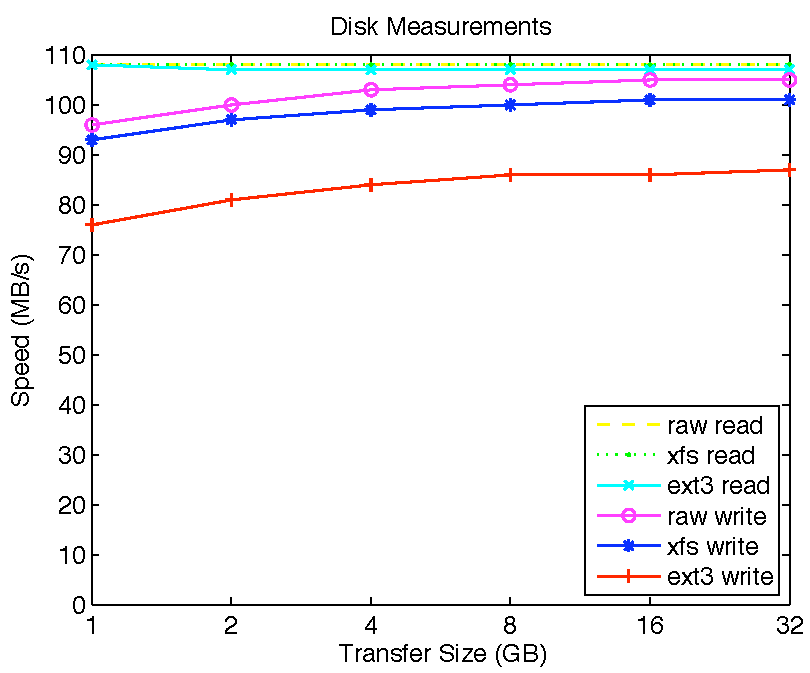
\includegraphics[height=2.5in]{fig_disk_measurements.pdf}
   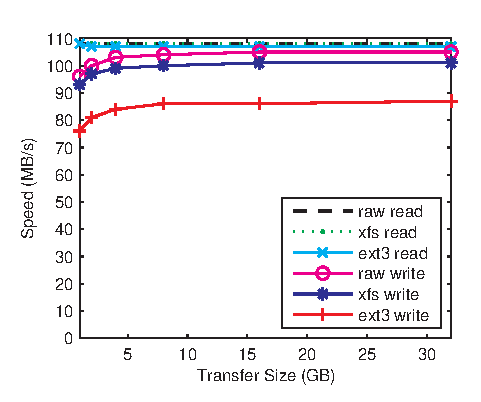
\includegraphics[height=2.5in]{fig_disk_measurements.eps}
%  }

\end{center}
\minicaption{Disk read and write measurements for a Seagate Barracuda drive}
{While read performance is consistently high across all systems,
  writes are slower, and \texttt{ext3} writes in particular are around
  20\% slower than raw device writes.}  

\label{fig:disk_measurements}
\end{figure}
}



%Our results show that Gigabyte-sized writes can be up to 32 MB/s
%slower than reads.  On the raw partition, this difference is smaller
%and becomes insignificant as the transfer size increases.  However, on
%ext3 and to a lesser extent on xfs, these differences become smaller
%but still persist for larger transfer sizes.

%Using the above results, we settled on XFS for use in all our
%subsequent experiments to get the fastest speeds, and a file size of
%4~GB per node to both achieve fast disk speeds and be able to keep all
%our intermediate data in memory.
The 108~MB/s value, and the \texttt{dd} measurements discussed above,
are for the first disk zone.
Modern disks have multiple zones, each with a different
data-per-track value and, thus, media transfer rate~\cite{Schindler02local}.
When measuring an XFS filesystem on a partition covering the entire disk,
read speeds remained consistent at 108 MB/s, but write speeds fluctuated
across a range of 92-102 MB/s with an average of 97 MB/s over 10 runs.
In reporting ``optimal'' values for experiments with our cluster, we
use 108~MB/s and 97~MB/s for the disk read and write speeds, respectively.

%However, these maximum transfer speeds also depend on the
%location of the data on disk -- the outer zones of a disk pack more
%sectors per track, allowing for faster data transfers than the zones
%that are closer to the spindle.

%Older, well-used filesystems may also be affected by fragmentation,
%which can interrupt sequential transfers with otherwise unnecessary
%disk seeks.  These issues can be solved by wiping and repartitioning
%the disks.  Therefore, we avoid dealing with fragmentation in our
%model.


\minorsection{Network bandwidth for applications}
Although a full-duplex 1~Gbps Ethernet link could theoretically
transfer 125~MB/s in each direction, maximum achievable data transfer
bandwidths are lower due to unavoidable protocol overheads.
Using the \texttt{iperf} tool with the maximum kernel-allowed 256~KB TCP
window size, we measured sustained bandwidths between two machines of
approximately 112.5 MB/s, which is in line with expected best-case
data bandwidth.
However, we observed lower bandwidths with more nodes in the all-to-all
pattern used in map-reduce jobs.
For example, in a 5--16 node all-to-all network transfer, we observed
102--106~MB/s aggregate node-to-node bandwidths over any one link.
These lower values are caused by NewReno's known slow convergence on
using full link bandwidths on high-speed networks~\cite{rapid-tcp}.
Such bandwidth reductions under some communication patterns may make
the use of a single network bandwidth ($N$) inappropriate for some environments.
For evaluating data-intensive computing on our cluster,
we use a conservative value of $N=110$~MB/s.

We also ran experiments using the newer CUBIC~\cite{cubic-tcp} congestion
control algorithm, which is the default on Linux 2.6.26 and is tuned to
support high-bandwidth links.
It achieved higher throughput (up to 115 MB/s per node with 10 nodes), but
exhibited significant unfairness between flows, yielding skews in
completion times of up to 86\% of the total time.
CUBIC's unfairness and stability issues are known and are prompting
continuing research toward better algorithms~\cite{rapid-tcp}.
%as a single speed.  However, since we do not have an implementation of
%better congestion control algorithms (e.g. RAPID~\cite{rapid-tcp}) for
%Linux, nor a more complex model that takes into account the high variability
%of NewReno and CUBIC, we use a conservative 110~MB/sec of network throughput
%with the understanding that we are overestimating the bandwidth achievable.
